\documentclass{beamer}
\setbeamertemplate{navigation symbols}{}

\usepackage{datetime2}
\usepackage{booktabs}
\usepackage{graphicx}

\graphicspath{{../code/data/}{../code/model/}{../code/work/}{../images/}}
\DeclareGraphicsExtensions{.pdf,.eps,.png}


\begin{document}

\begin{frame}[fragile]
	\vspace{0.3\textheight}
	
	\begin{center}
		\large
		On-demand public transport \\
		\small
		{\color{gray} is making us mobile }
	\end{center}
	
	\vspace{\stretch{100}}

	\tiny
	R.~Andreev \verb|<andreevr@ethz.ch>|, \today
	\hfill
	\tiny\color{lightgray}\hfill{\DTMnow}
\end{frame}


\begin{frame}
	NYC TLC taxi data, May 2016:
	
	{\ }
	
	\resizebox{\textwidth}{!}{\begin{tabular}{llllllllll}
\toprule
             pickup &             dropoff &     xa\_lat &     xa\_lon &     xb\_lat &     xb\_lon & n & meters & seconds &      \$ \\
\midrule
2016-05-01 00:00:04 & 2016-05-01 00:06:22 &  40.839329 & -73.940842 &  40.850304 & -73.932976 & 1 &   1368 &     378 &    7.3 \\
2016-05-01 00:00:07 & 2016-05-01 00:01:58 &  40.859612 & -73.930199 &  40.863338 & -73.929977 & 1 &    531 &     111 &    4.8 \\
2016-05-01 00:00:14 & 2016-05-01 00:14:37 &  40.828629 & -73.942215 &  40.763519 & -73.996788 & 1 &  10783 &     863 &   22.3 \\
2016-05-01 00:00:25 & 2016-05-01 00:04:37 &  40.807968 & -73.945488 &  40.804539 & -73.955505 & 1 &   1287 &     252 &    7.3 \\
2016-05-01 00:00:28 & 2016-05-01 00:23:02 &  40.785992 & -73.948799 &  40.763748 & -73.988724 & 1 &   6598 &    1354 &  23.16 \\
2016-05-01 00:00:30 & 2016-05-01 00:05:19 &  40.785416 & -73.949669 &  40.776234 & -73.952744 & 1 &   1255 &     289 &   8.16 \\
                ... &                     &            &            &            &            &   &        &         &        \\
\bottomrule
\end{tabular}

}
	
	\vspace{2\baselineskip}
	
	How many minibuses could meet the same demand?
\end{frame}


\begin{frame}[t]
	From trip endpoints and travel time
	we infer traffic conditions:
	
	\begin{center}
		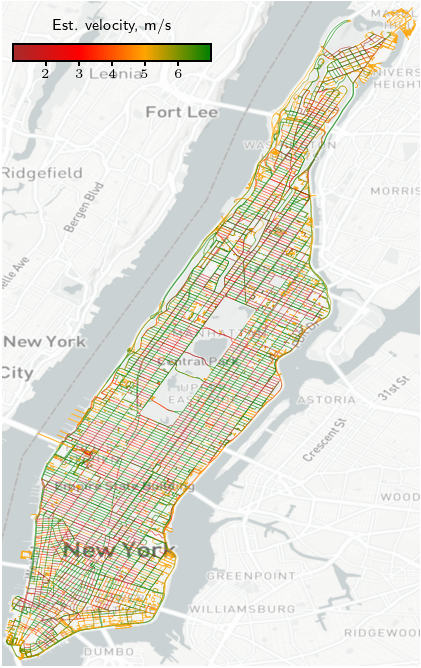
\includegraphics[width=0.40\textwidth]{20210613-GraphWithLag/b_train/v1/lag/H=18/UTC-20210615-132827/train/velocity_i=9.png}
	\end{center}
	
	Use this for quickest routes.
\end{frame}


\begin{frame}[t]
	Case study: 
	\begin{itemize}
	\item
		100 requests during 18:00--18:17
		within 1km of Times Square
	\item
		Allow -2min/+5min pickup and +10min dropoff windows
	\item
		Assume good traffic conditions
	\end{itemize}
	
	{\ }
	
	Excess travel times (wrt quickest route) computed by optimizer:
	
	\only<2>{%
		\begin{center}
			\small
			10 single-passenger taxis
			
			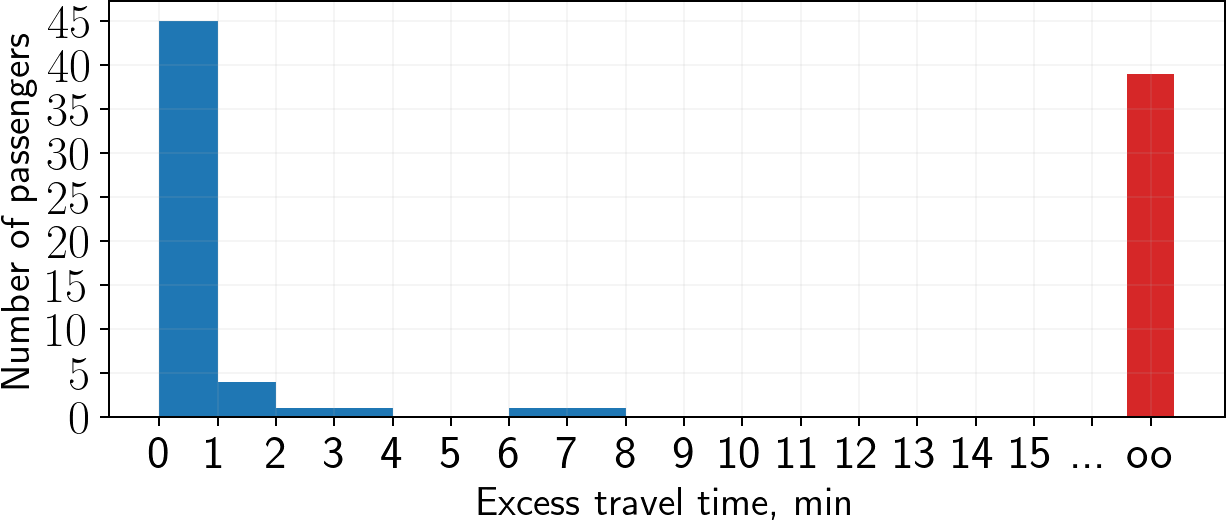
\includegraphics[width=0.8\textwidth]{20210616-OPT1/c_grid_study0/UTC-20210619-074952/c_grid_visualize/8/excess_travel_time_hist}
		\end{center}
	}%
	\only<3>{%
		\begin{center}
			\small
			10 minibuses of capacity 8
			\\
			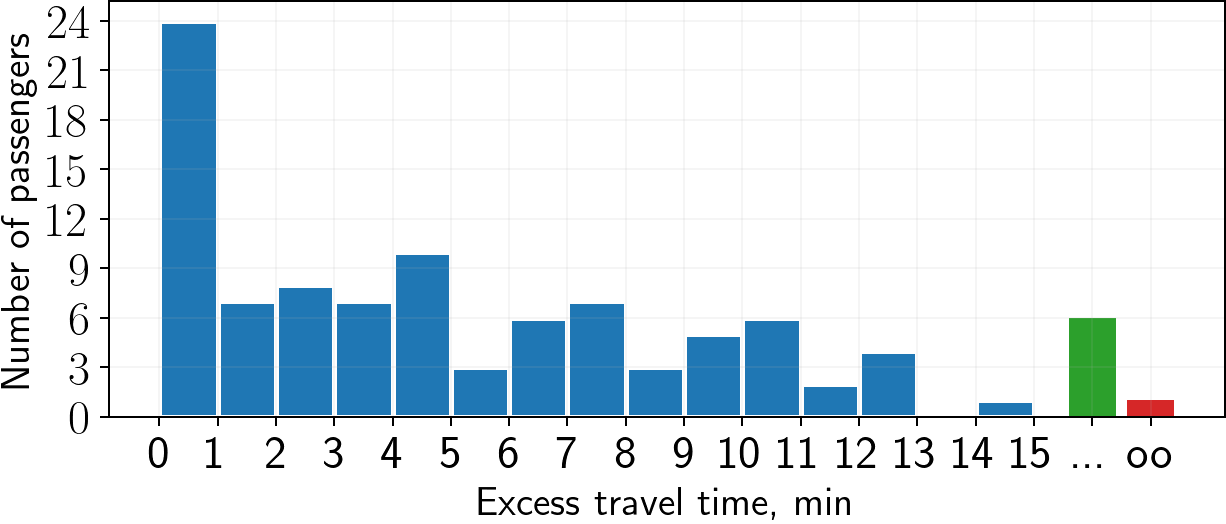
\includegraphics[width=0.8\textwidth]{20210616-OPT1/c_grid_study0/UTC-20210619-074952/c_grid_visualize/9/excess_travel_time_hist}
		\end{center}
		
		Hence:
		20 taxis $\approx$ 10 minibuses,
		if allow detours.
	}
\end{frame}


\begin{frame}[t]
	Assume
	\begin{itemize}
	\item A certain proportion of minibus takers.
	\item Excess travel times in dollars according to 2019 income census.
	\item Prefer minibus if income/min $<$ expected excess travel time.
	\end{itemize}
	
	\only<2>{%
		\begin{center}
			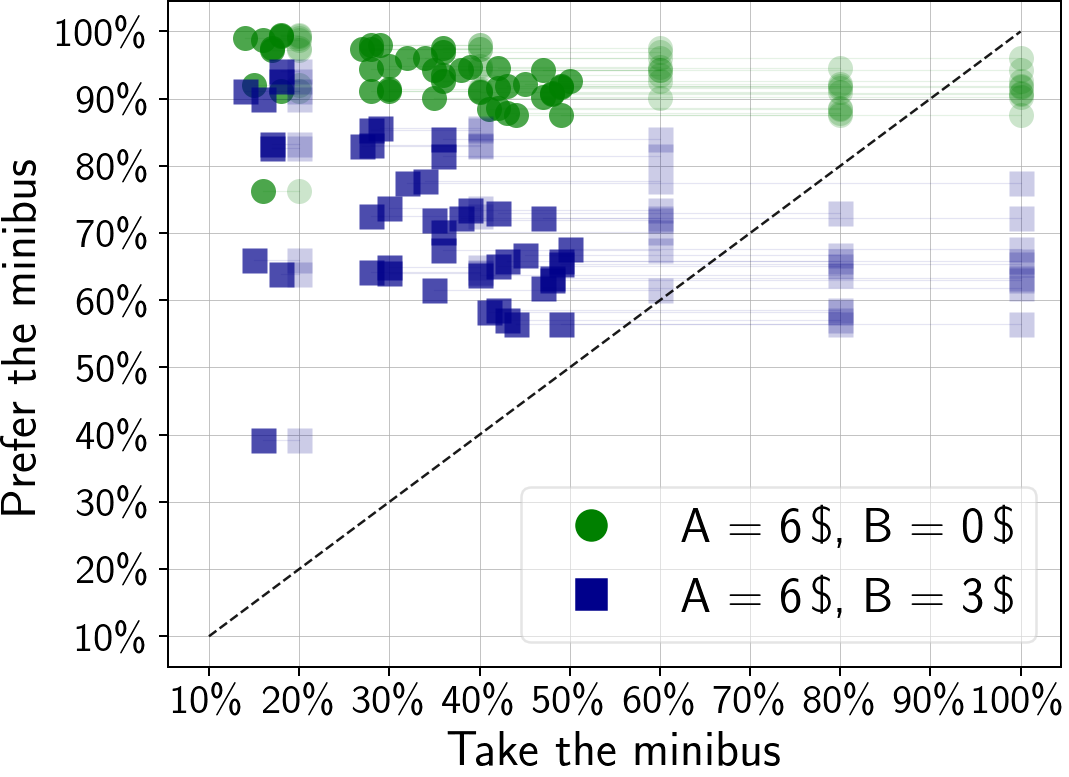
\includegraphics[width=0.55\textwidth]{20210616-OPT1/c_grid_study1b/UTC-20210623-191629/e_evo_plots/evo__graph_h=6__graph_ttt_factor=3}
		\end{center}	
		
		\small
		
		Assume bad traffic conditions (6pm traffic).
		\\
		Minibuses can meet only half of the demand.
		
		\color{gray}
		Faint: imposed fraction of bus takers.
		Solid: net the unserviced requests.
		\\
		A = taxi price, B = minibus ride price
	}%
		
	\only<3>{%
		\begin{center}
			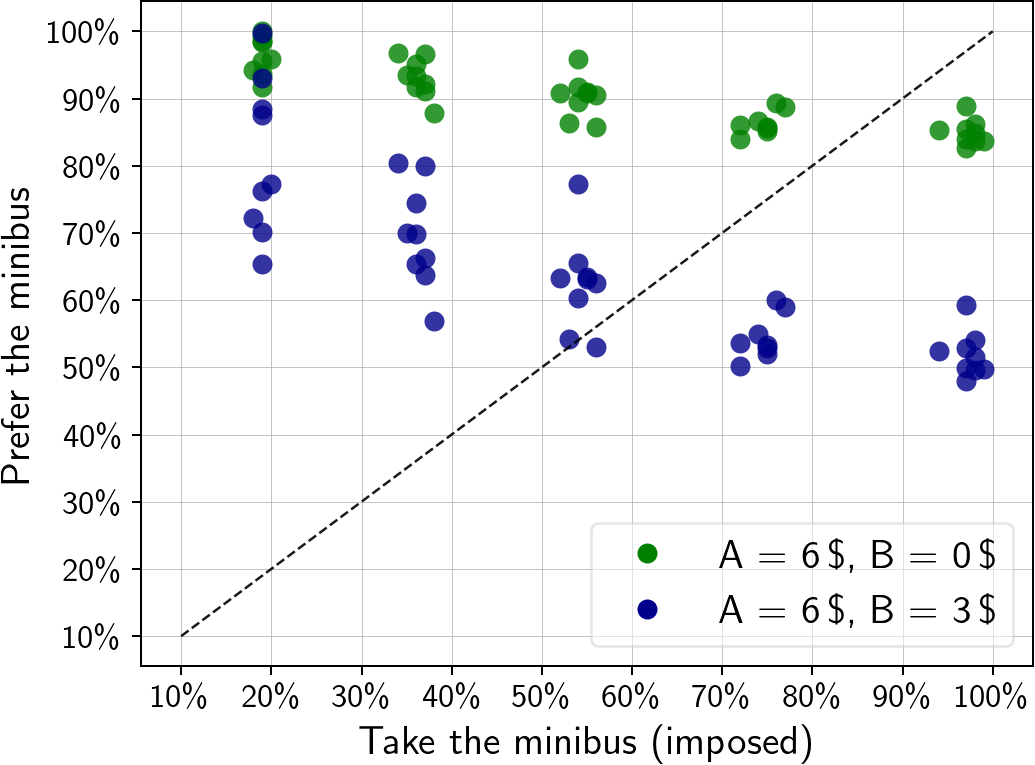
\includegraphics[width=0.55\textwidth]{20210616-OPT1/c_grid_study1/UTC-20210621-232339/e_evo_plots/evo}%
		\end{center}
		
		\small
		
		Assume traffic improves (6pm $\leadsto$ 6am)
		as more people take the minibus.
		\\
		Equilibrium at 50-90\% bus takers, depending on the price.
	}
\end{frame}

\begin{frame}

	\vspace{5\baselineskip}
	
	The paradigm shift is feasible -- if it improves the traffic conditions.
	

	\vspace{\stretch{100}}

	
	\small
	Details:
	\url{http://bit.ly/optimum-2021}
\end{frame}
\end{document}


